%TODO: Раздел второй - ЭЛЕКТРОМАГНИТНЫЕ ПЕРЕХОДНЫЕ ПРОЦЕССЫ ПРИ СОХРАНЕНИИ СИММЕТРИИ ТРЕХФАЗНОЙ ЦЕПИ
\chapter{Переходный процесс в простейших трехфазных цепях}
\label{chap:3 perehodnyi_protcess_v_prosteishikh_trekhfaznykh_tcepiakh}

\section{Постановка задачи и ее ограничения}
\label{sec:3-1 postanovka_zadachi_i_ee_ogranicheniia}

Симметричную трехфазную цепь с сосредоточенными активными сопротивлениями и индуктивностями при отсутствии в ней трансформаторных связей условимся называть \so{простейшей} трехфазной цепью.

Электромагнитный переходный процесс в такой цепи рассмотрим сначала при условии, что ее питание осуществляется от источника, сопротивление которого равно нулю и его напряжение, изменяясь с постоянной частотой, имеет неизменную амплитуду\footnote{Применение чувствительного и быстродействующего автоматического регулировании возбуждения генераторов дополнительно способствует принятию указанного предположения.}. Обычно его называют источником бесконечной  мощности.

Включение в схему такого источника, вообще говоря, соответствует теоретическому пределу, когда изменение внешних условий не влияет на работу самого источнику. Практически это имеет место, например, при коротких замыканиях в относительно маломощных электрических установках или протяженных сетях, питаемых от крупных энергетических систем (см.~\colorbox{red}{гл. 17}).

С исследованием переходных процессов в подобных условиях читатель знаком из курса теоретических основ электротехники. Поэтому задачей данной главы является кратко напомнить основные выводы такого исследования, отметить особенности многофазной цепи по сравнению с однофазной, привести некоторые упрощенные приемы расчета и обратить внимание на влияние ряда факторов.

\section{Трехфазное короткое замыкание в неразветвленной цепи}
\label{sec:3-2 trekhfaznoe_korotkoe_zamykanie_v_nerazvetvlennoi_tcepi}

Обратимся к рис.~\ref{ris:3-1 simple_3_phase_circut}, на котором представлена простейшая симметричная трехфазная цепь. В ней условно принято, что на одном ее участке имеется взаимоиндукция между фазами, а на другом она отсутствует. Цепь присоединена к источнику синусоидального напряжения с неизменными амплитудой и частотой.

Рассмотрим переходный процесс, вызванный включением выключателя \textit{B}, за которым сделана закоротка, что равносильно возникновению металлического трехфазного короткого замыкания между двумя участками данной цепи.

\begin{figure}[h]
	\center{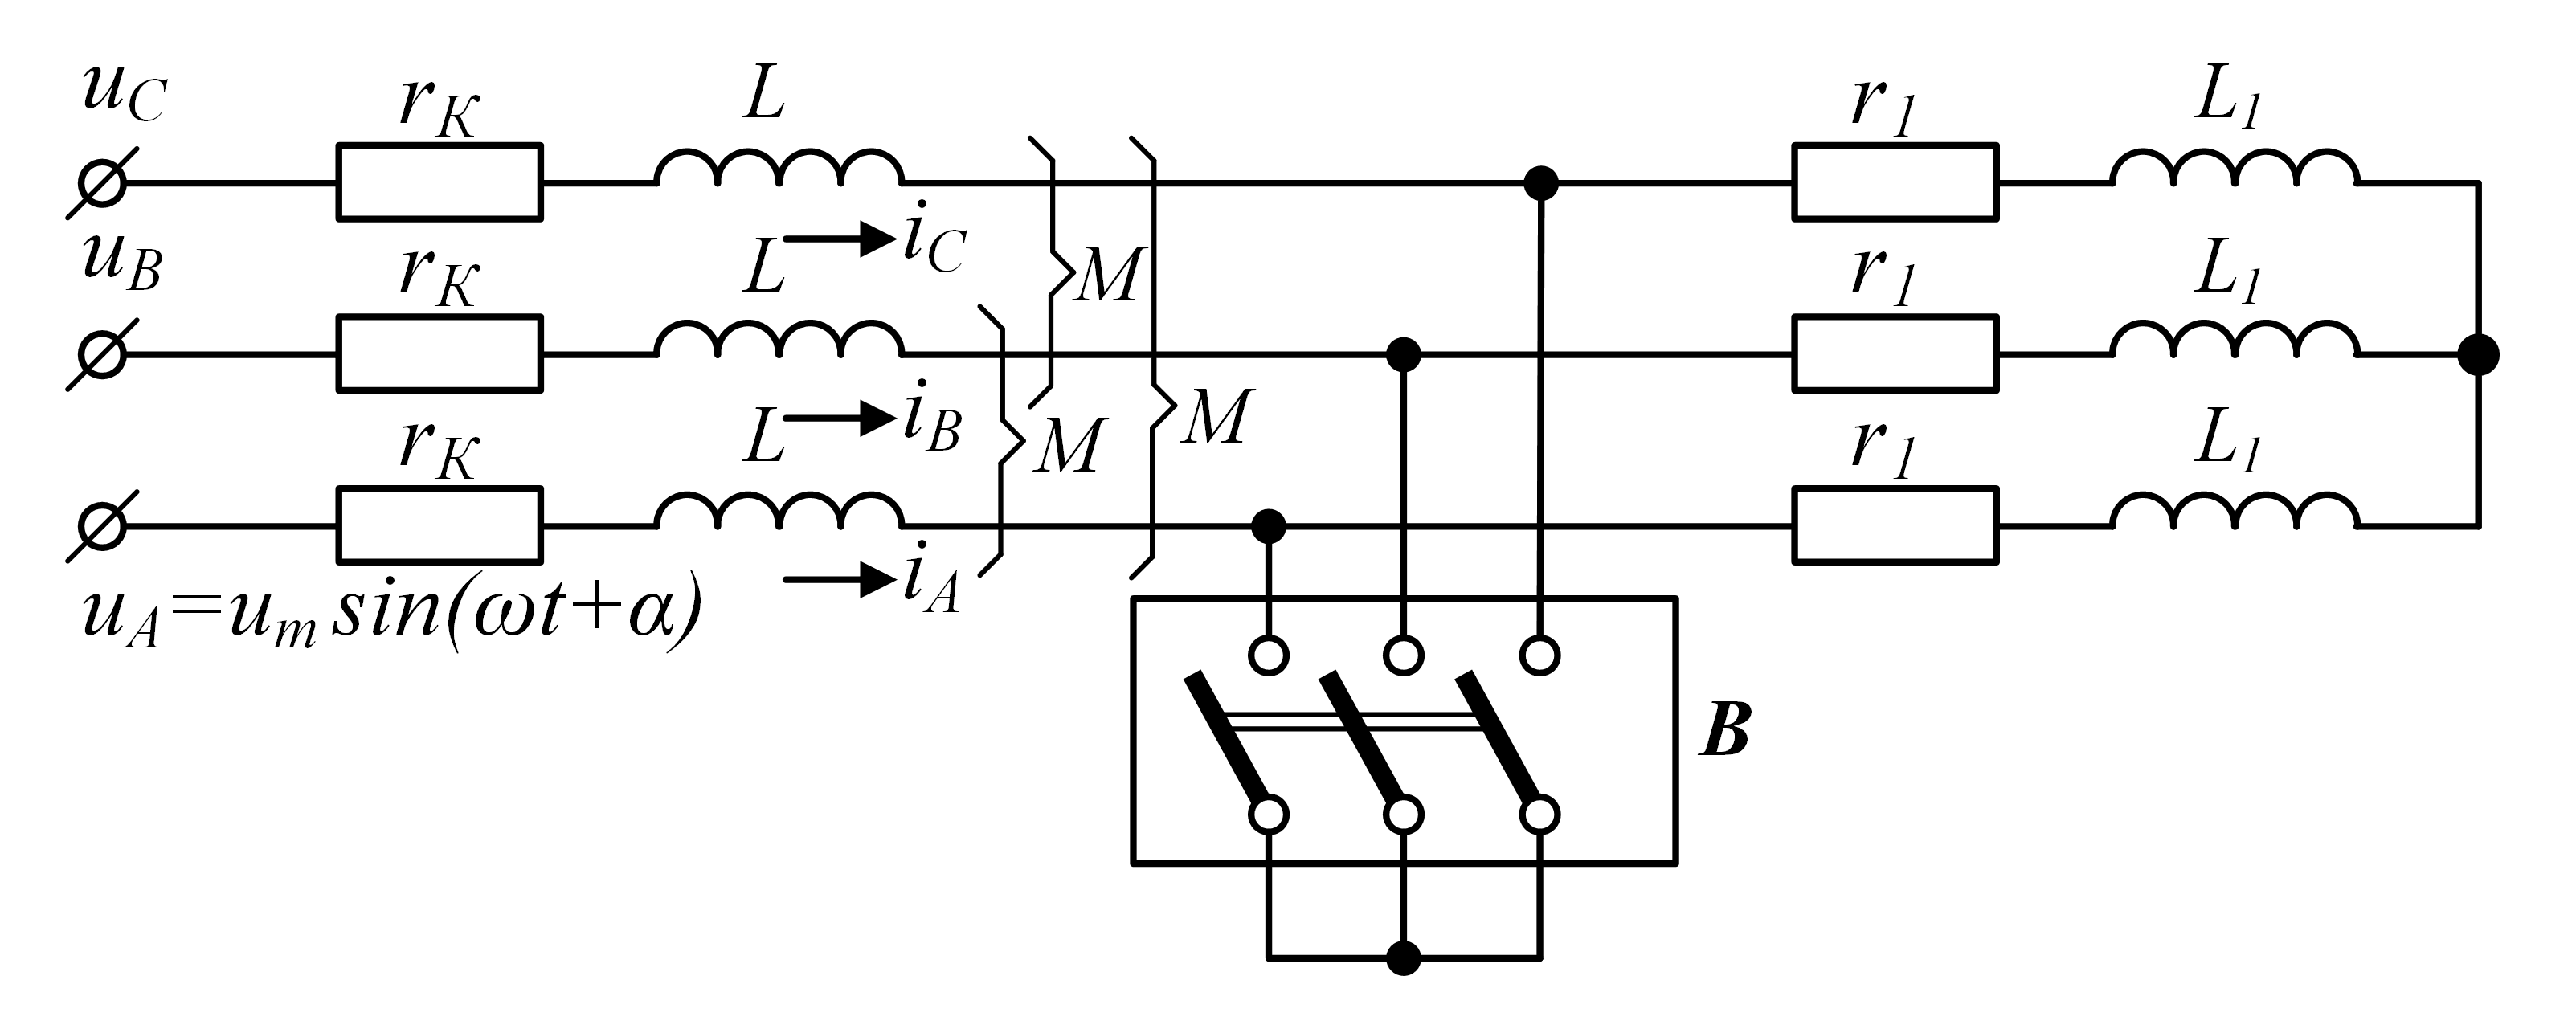
\includegraphics[width=0.9\linewidth]{pic/3-1}}
	\caption{Простейшая трехфазная электрическая цепь.}
	\label{ris:3-1 simple_3_phase_circut}
\end{figure}

Пусть векторы $ \overset{\;.}{U}_A $, $ \overset{\;.}{U}_B $, $ \overset{\;.}{U}_C $, $ \overset{\;.}{I}_A $, $ \overset{\;.}{U}_B $, $ \overset{\;.}{U}_C $ (рис.~\ref{ris:3-2 diagram})
характеризуют предшествующий режим рассматриваемой цепи, а вертикаль \textit{tt} является неподвижной линией времени, т.~е. мгновенные значения отдельных величии определяются проекциями на эту линию соответствующих вращающихся векторов. Момент возникновения короткого замыкания будем фиксировать значением угла $ \alpha $ (т.~е. \so{фазой включения}) между вектором напряжения фазы \textit{A} и горизонталью. (рис.~\ref{ris:3-2 diagram}.

После включения выключателя \textit{В} цепь рис.~\ref{ris:3-1 simple_3_phase_circut} распадается на два независимых друг от друга участка. Участок с $ r_1 $ и $ L_1 $ оказывается зашунтированным коротким замыканием и ток в нем будет поддерживаться лишь до тех пор, пока запасенная в индуктивности $ L_1 $ энергия магнитного потока не перейдет в тепло, поглощаемое активным сопротивлением $ r_1 $.

Дифференциальное уравнение равновесия в каждой фазе этого участка имеет вид:

\begin{equation}
	0 = ir_1 + L_1 \frac{di}{dt}.
	\label{eq:3-1 diff_ur}
\end{equation}

Его решение общеизвестно:

\begin{equation}
	i = i_0 e^{-t / T_{\text{а}1}}; %TODO: Проверить формулу, какая-то черка в степени
	\label{eq:3-2 diff_solve}
\end{equation}

оно показывает, что здесь имеется лишь свободный ток, который затухает по экспоненте с постоянной времени

\begin{equation}
	T_{\text{а}1} = \frac{L_1}{r_1} = \frac{x_1}{\omega r_1}, \textit{~сек}.
	\label{eq:3-3 T_a1}
\end{equation}

Начальное значение свободного тока в каждой фазе зашунтированного участка цепи, очевидно, равно предшествовавшему мгновенному значению тока, поскольку в цепи с индуктивностью не может произойти внезапного (скачком) изменения тока. В общем случае свободные токи в фазах различны, хотя их затухание, разумеется, происходит с одной и той же постоянной времени. В одной из фаз свободный ток может вообще отсутствовать, если в момент возникновения короткого замыкания предшествовавший ток в этой фазе проходил через нуль; при этом свободные токи в двух других фазах будут одинаковы по величине, но противоположны по направлению.

На рис.\colorbox{red}{3-3} слева приведены кривые изменения фазных токов в зашунтированном участке рассматриваемой цени, с учетам, что короткое замыкание произошло в момент, отвечающий положению векторов на рис.~\ref{ris:3-2 diagram}.

\begin{floatingfigure}[lflt]{0.45\linewidth}
	\centering
	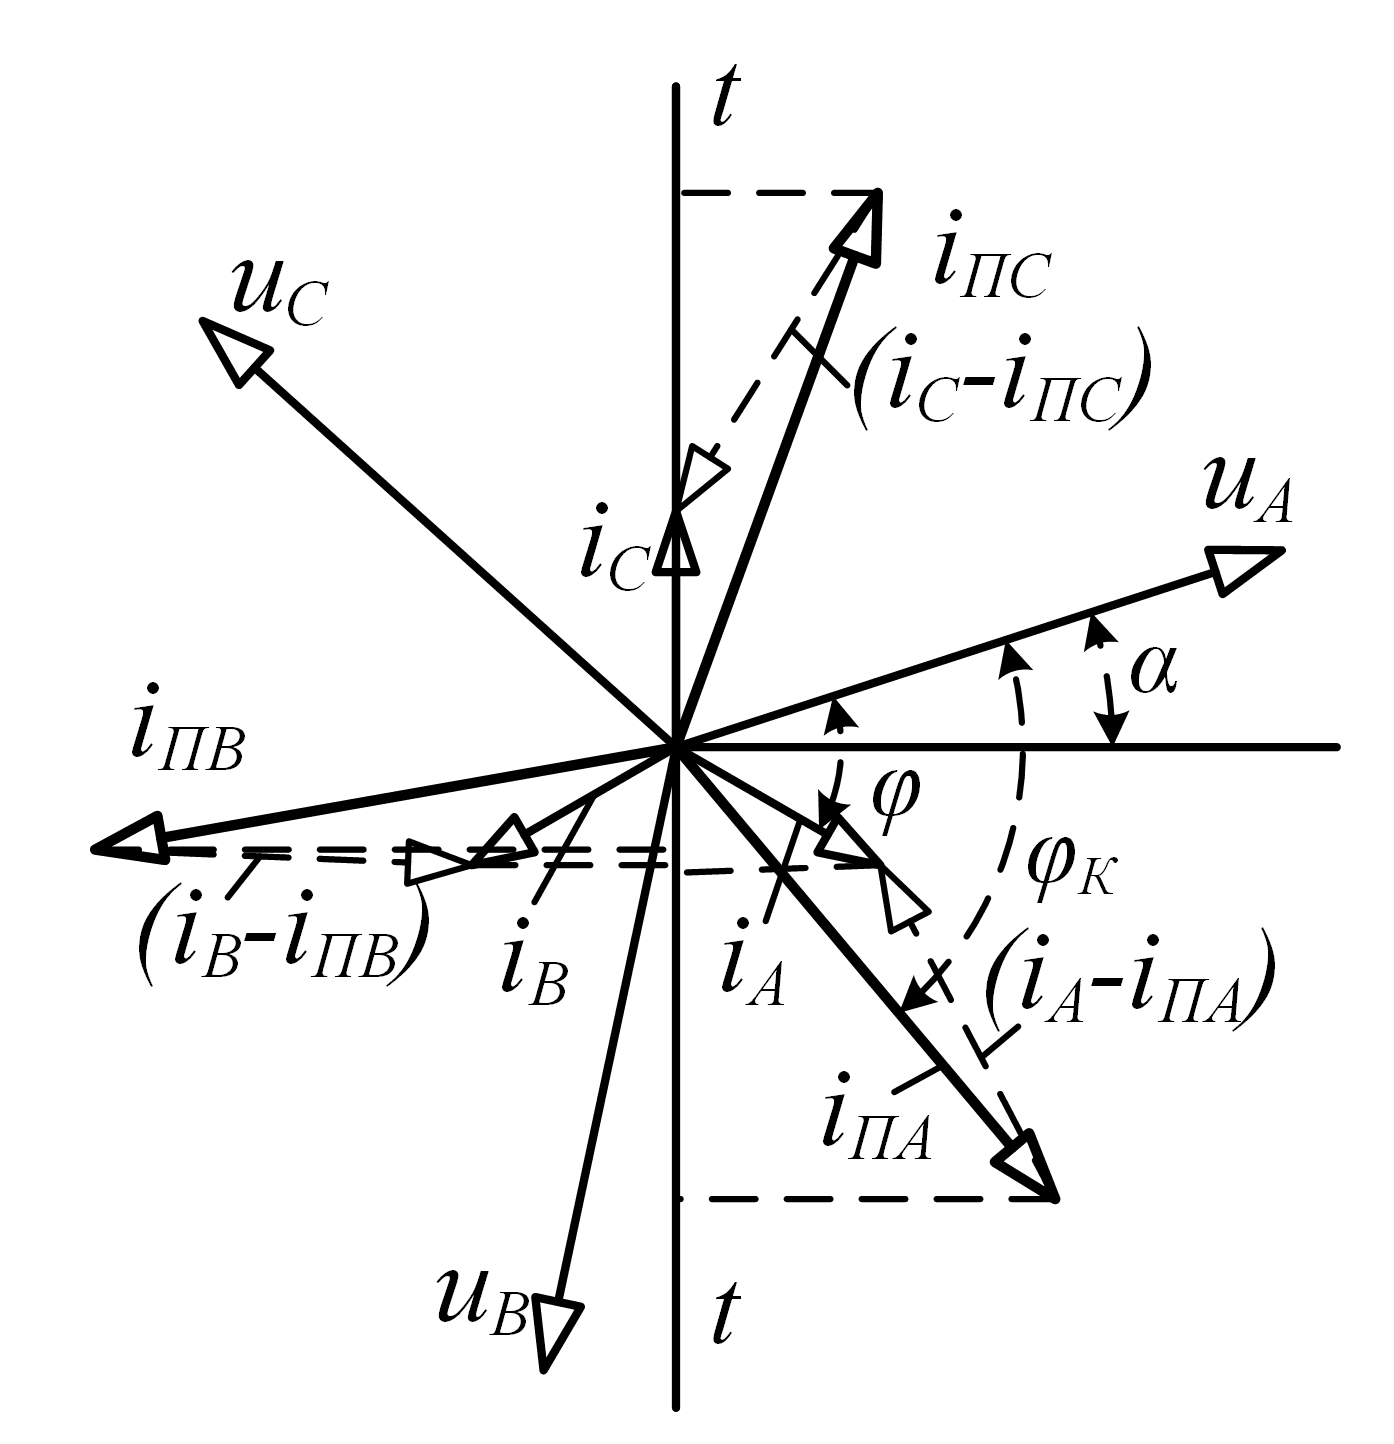
\includegraphics[width=0.40\linewidth]{pic/3-2}
	\caption{Векторная диаграмма для начального момента трехфазного короткого замыкания.}
	\label{ris:3-2 diagram}
\end{floatingfigure}

\begin{small}
	Напомним, что подкасательная в любой точке экспоненты\footnote{Обычно используют начальную часть экспоненты, где скорость изменения соответствующей величины больше и поэтому можно точнее провести касательную.} в принятом для оси времени масштабе дает значение постоянной времени, с которой происходит изменение экспоненты (рис. \colorbox{red}{3-3}). Имея в виду, что при $ t = T_{\text{а}} $ значение $ e^{-1} = 0,368 $, постоянную $ T_{\text{а}} $ обычно трактуют как время, в течение которого переменная величина снижается до 0,368 своего начального значения; при этом за начальную может быть принята любая точка кривой.
	
\end{small}

%TODO: Рисунок оказывается перед 3-2 ??!!
\begin{figure}
	\center{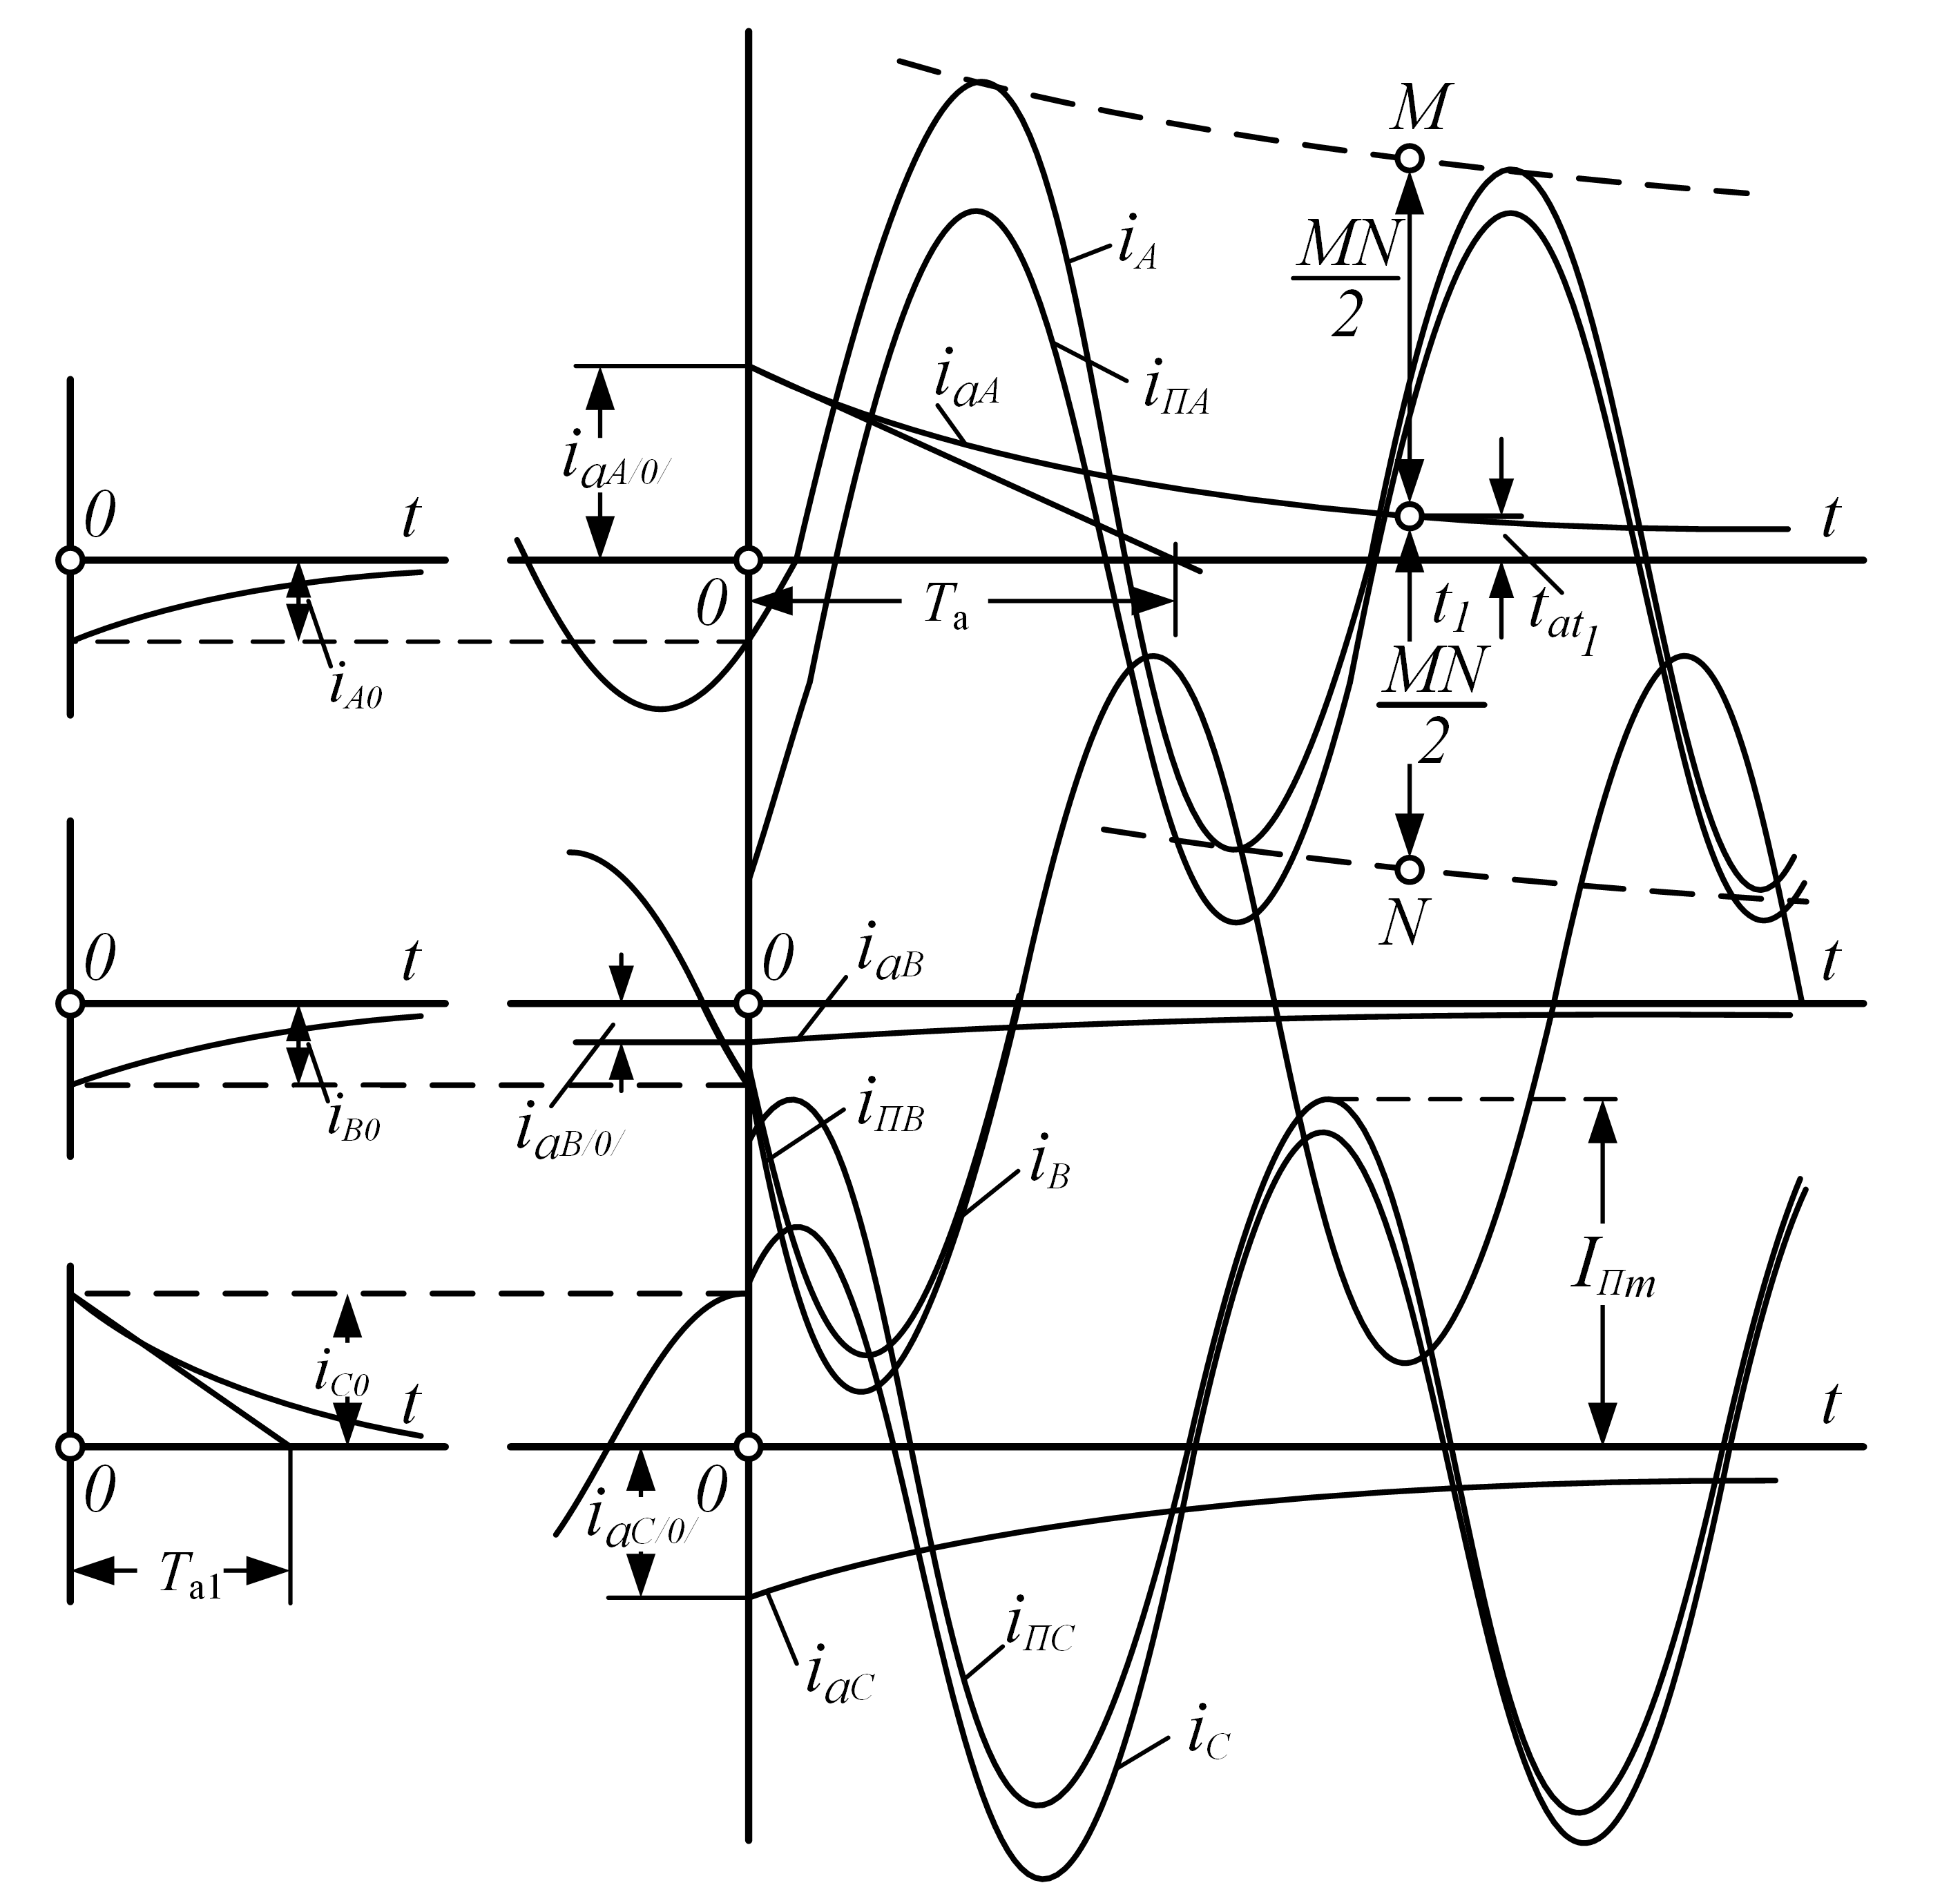
\includegraphics[width=0.85\linewidth]{pic/3-3}}
	\caption{Осциллограммы токов в фазах при внезапном трехфазном коротком замыкании в простейшей электрической цепи.}
	\label{ris:3-3}
\end{figure}

Перейдем теперь к участку цепи, который остался присоединенным к источнику. Здесь помимо свободного тока будет новый принужденный ток, величина которого, очевидно, больше предыдущего и сдвиг по фазе которого в общем случае иной. Допустим, что векторы $ I_{\text{П}A} $, $ I_{\text{П}B} $, $ I_{\text{П}C} $ (рис.~\ref{ris:3-2 diagram}) отвечают новому установившемуся режиму данного участка цепи.

Дифференциальное уравнение равновесия для любом фазы, например фазы \textit{А}, этого участка

\begin{equation*}
	u_A = i_A r_{\text{К}} + L \frac{di_A}{dt} + M \frac{di_B}{dt} + M \frac{di_C}{dt},
\end{equation*}

имея ввиду, что $ (i_B + i_C) = -i_A $, можно представить (опуская индекс фазы) как

\begin{equation}	
	u = i r_{\text{К}} + L_{\text{К}} \frac{di}{dt},
	\tag{\ref*{eq:3-1 diff_ur}а}
	\label{eq:3-1a u}
\end{equation}

где $ L_{\text{К}} = (L - M) $ --- результирующая индуктивность фазы, т.~е. индуктивность с учетом влияния двух других фаз.

Решение (\ref{eq:3-1a u}) имеет вид:

\begin{equation}	
	i = \frac{U_m}{z_{\text{К}}} sin(\omega t + \alpha - \varphi_{\text{К}}) + i_{\text{а} | 0 |} e^{-t / T_{\text{а}}}
	\tag{\ref*{eq:3-2 diff_solve}а}
	\label{eq:3-2a i}
\end{equation}

где $ z_{\text{К}} $ --- полное сопротивление присоединенного к источнику участка цепи или. короче, цепи короткого замыкания;

$ \varphi_{\text{К}} $ --- угол сдвига тока в этой цепи;
	
$ T_{\text{a}} $ --- постоянная времени цепи короткого замыкания, определяемая по (\ref{eq:3-3 T_a1}), где вместо $ L_1 $, $ x_1 $, $ r_1 $ следует ввести $ L_{\text{К}} $, $ x_{\text{К}} $, $ r_{\text{К}} $.

Первый член правой части (\ref{eq:3-2a i}) представляет периодическую слагающую тока, которая при рассматриваемых условиях является принужденным током с постоянной амплитудой $ I_{\text{П}m} = U_m / z_{\text{К}} $. Соответственно второй член представляет, как и раньше, затухающий по экспоненте свободный ток; его называют также апериодической слагающей тока. Начальное значение этой слагающей определяется из начальных условий, т.~е.

% В этом месте в книге опечатка, формула названа 3-3, нумерация дальше отличается
\begin{equation}
	i_0 = i_{\text{п}~/0/} + i_{\text{а}~/0/},
	\label{eq:3-4 i_0}
\end{equation}

откуда после подстановки соответствующих выражений имеем:

\begin{equation}
	i_{\text{а}|0|} = I_m sin(\alpha - \varphi) - I_{\text{П}m} sin(\alpha - \varphi_{\text{К}}).
	\label{eq:3-5 i_a0}
\end{equation}

Поскольку токи $ i_{\text{П}} $, $ i_0 $ являются проекциями векторов $ \overset{\;.}{I}_{\text{П}m} $ и $ \overset{\;.}{I}_m $ на линию времени, то ток $ 	i_{\text{а}|0|} $ также можно рассматривать как проекцию вектора $ (\overset{\;.}{I}_m - \overset{\;.}{I}_{\text{П}m} $ на ту же линию (рис.~\ref{ris:3-2 diagram}). В зависимости от фазы включения $ \alpha $ начальное значение тока $ 	i_{\text{а}|0|} $ может изменяться от возможной наибольшей величины, когда вектор $ (\overset{\;.}{I}_m - \overset{\;.}{I}_{\text{П}m} $ параллелен линии времени, до нуля, когда этот вектор нормален к ней. В трехфазной системе такие частные условия, разумеется, могут быть лишь в одной из фаз.

%TODO: Рисунок 3-4

На рис. \colorbox{red}{3-3} справа представлены кривые изменения токов в фазах рассматриваемого участка при трехфазном коротком замыкании. Как видно, чем больше апериодическая слагающая тока, тем больше смещение кривой полного тока относительно оси времени. Эту слагающую можно рассматривать как криволинейную ось симметрии кривой полного тока, из которой ее легко выделить. Для этого нужно сначала провести огибающие по максимальным положительным и отрицательным значениям заданной кривой тока (см. пунктирные линии у кривой тока фазы \textit{А} на \colorbox{red}{рис. 3-3}). Каждая точка кривой апериодической слагающей лежит посредине вертикального отрезка между этими огибающими.

Из (\colorbox{red}{3-4}) и рис. \colorbox{red}{3-2} следует, что наибольшее значение апериодической слагающей тока определяется не только фазой включения, но также предшествующим режимом цепи. Так, например, при отсутствии предшествующего тока в данной цепи величина 
при отсутствии величина $ i_{\text{а}/0/} $ может достигать амплитуды периодической слагающей, если в момент короткого замыкания эта слагающая проходит через свой положительный или отрицательный максимум (рис.\colorbox{red}{3-4}). Обычно этот случай рассматривается как расчетный\footnote{Хотя возможны частные случаи, когда начальное значение апериодической слагающей тока превышает амплитуду периодической слагающей.}.

Важно отметить, что фаза включения, при которой возникает наибольшее значение апериодической слагающей, еще не предопределяет того, что именно при ней будет максимум мгновенного значения полного тока. В самом деле, из (\ref{eq:3-2a i}) и (\ref{eq:3-5 i_a0}) при отсутствии предшествующего тока ($ I_m = 0 $) следует, что полный ток в цепи короткого замыкания является функцией двух независимых переменных: времени $ t $ и фазы включения $ \alpha $ и выражается уравнением








